\documentclass[conference]{IEEEtran}
%
%% article_syscon.tex
%% V1.4
%% 2012/12/27
%% by Smail Rahmoun

%% Support sites:
%% http://www.michaelshell.org/tex/ieeetran/
%% http://www.ctan.org/tex-archive/macros/latex/contrib/IEEEtran/
%% and
%% http://www.ieee.org/

% Add the compsoc option for Computer Society conferences.
%
% If IEEEtran.cls has not been installed into the LaTeX system files,
% manually specify the path to it like:
% \documentclass[conference]{../sty/IEEEtran}


% Some very useful LaTeX packages include:
% (uncomment the ones you want to load)


% *** MISC UTILITY PACKAGES ***
%
%\usepackage{ifpdf}
% Heiko Oberdiek's ifpdf.sty is very useful if you need conditional
% compilation based on whether the output is pdf or dvi.
% usage:
% \ifpdf
%   % pdf code
% \else
%   % dvi code
% \fi
% The latest version of ifpdf.sty can be obtained from:
% http://www.ctan.org/tex-archive/macros/latex/contrib/oberdiek/
% Also, note that IEEEtran.cls V1.7 and later provides a builtin
% \ifCLASSINFOpdf conditional that works the same way.
% When switching from latex to pdflatex and vice-versa, the compiler may
% have to be run twice to clear warning/error messages.

% *** CITATION PACKAGES ***
%
\usepackage{cite}

% *** GRAPHICS RELATED PACKAGES ***
%
\ifCLASSINFOpdf
\usepackage[pdftex]{graphicx}
  % declare the path(s) where your graphic files are
  % \graphicspath{{../pdf/}{../jpeg/}}
  % and their extensions so you won't have to specify these with
  % every instance of \includegraphics
  % \DeclareGraphicsExtensions{.pdf,.jpeg,.png}
\else
  % or other class option (dvipsone, dvipdf, if not using dvips). graphicx
  % will default to the driver specified in the system graphics.cfg if no
  % driver is specified.
\usepackage[dvips]{graphicx}
  % declare the path(s) where your graphic files are
  % \graphicspath{{../eps/}}
  % and their extensions so you won't have to specify these with
  % every instance of \includegraphics
  % \DeclareGraphicsExtensions{.eps}
\fi


% *** MATH PACKAGES ***
%
\usepackage[cmex10]{amsmath}


% *** SPECIALIZED LIST PACKAGES ***
%
\usepackage{algorithmic}

% *** ALIGNMENT PACKAGES ***
%
\usepackage{array}

% *** SUBFIGURE PACKAGES ***
\ifCLASSOPTIONcompsoc
  \usepackage[caption=false,font=normalsize,labelfont=sf,textfont=sf]{subfig}
\else
  \usepackage[caption=false,font=footnotesize]{subfig}
\fi

% *** FLOAT PACKAGES ***
%
%\usepackage{fixltx2e}
%\usepackage{stfloats}
\usepackage{dblfloatfix}

% *** PDF, URL AND HYPERLINK PACKAGES ***
\usepackage{url}

% correct bad hyphenation here
\hyphenation{op-tical net-works semi-conduc-tor}

\begin{document}
\title{Using NSGA-II to compose model transformations alternatives }

%\author{\IEEEauthorblockN{Smail Rahmoun}
%\IEEEauthorblockA{Institute for Technological Research\\SystemX\\
%Palaiseau France\\
%Email: smail.rahmoun@irt-systemx.fr}
%\and
%\IEEEauthorblockN{Etienne Borde\\ and Laurent Pautet}
%\IEEEauthorblockA{TELECOM Paristech Institut\\
%LTCI-UMR 5141\\
%Paris, France\\
%Email: firstname.name@telecom-paristech.fr}}
 \author{\IEEEauthorblockN{
  Smail Rahmoun\IEEEauthorrefmark{1}\IEEEauthorrefmark{2},
  Etienne Borde\IEEEauthorrefmark{2},
  Laurent Pautet\IEEEauthorrefmark{2},
}

\IEEEauthorblockA{\IEEEauthorrefmark{1}Institute for Technological Research SystemX
                - 8, Avenue de la Vauve 91120 PALAISEAU\\
                % Palaiseau France\\
                firstname.lastname@irt-systemx.fr}

\IEEEauthorblockA{\IEEEauthorrefmark{2}Institut Telecom;TELECOM ParisTech; LTCI - UMR 5141
                - 46 rue Barrault, 75013 Paris, France\\
                firstname.lastname@telecom-paristech.fr}

}

\maketitle

\begin{abstract}
The size and complexity of modern systems is rapidly increasing. Meanwhile, the ability to understand and maintain such systems is decreasing almost as fast.
Model Driven Engineering promotes the automation of design activities by means of model transformations, enabling to cope with systems complexity. However, the design space produced by the composition of these model transformations is difficult to explore automatically. The main reason that make this exploration difficult is the size of the design space : the number of possible design choices grows exponentially with the number of model transformation alternatives.
This paper presents a MDA approach for design space exploration to deal with the ever-growing challenge of designing complex embedded systems. This approach allows the system architects to automatically select the most adequate model transformations compositions by using multi-objectives optimization evolutionary algorithms.

\end{abstract}

\IEEEpeerreviewmaketitle

\section{Introduction}
Nowadays, modern systems become more and more large and complex and therefore more difficult to develop and maintain. For example, embedded critical systems which are often built to accomplish specific functionalities, can integrate several buses, software and hardware components. To guarantee properties such as safety, availability and robustness makes the design of these systems very challenging.

Model Driven Engineering (MDE) proposes the use of models as the key assets in the development of such systems. Model transformations approach become one of the basic building blocks of MDE. Even though MDE is being successfully applied in many scenarios, it still needs appropriate mechanisms to handle the development of complex, large-scale systems. One such mechanism is a facility to make transformations reusable, so that we can apply them to different contexts. In this work, we use generic model transformation to model design alternatives of the system. This process will help us to predict non-functional properties (NFP) of a system before its development\cite{1291833}. This prediction can be exploited to drive decisions about which components should be used and how they should be connected so as to meet the NFP imposed on the design.

Moreover, an issue in modeling a system is that, the NFP could conflict\footnote{improving one property can have a negative impact on other properties} with each other. For example, improving the availability of a service is often done by replication of the service, which causes the increasing of the response time of these services\cite{Yu:2001:CLA:502059.502038}. Developing a system that satisfies at best all its NFP simultaneously is often not possible : improving a NFP of a system can deteriorate another NFP. As a consequence, system architects have to come up with several design alternatives and select the solutions which fulfils at best all NFP\cite{Coello98acomprehensive} simultaneously from all feasible alternatives. The selected solutions are called non-dominated solutions or Pareto optimal solutions : a solution x2 is non-dominated by another solution x1, if x2 matches or exceeds x1 in all objectives (NFP).

In order to obtain the set of Pareto optimal alternatives, some advanced multi-objective optimization evolutionary algorithms (MOEA) have been proposed. These algorithms apply some fitness evaluations and generic operators of variation. Thus, they are applicable to search spaces (e.g. design space) taking into account domain specific characteristics of the problem (e.g. prediction of NFP). MOEA also provides selection operators which guide the search towards interesting regions of the search space by (i) favorizing non-dominated solutions; and (ii) finding a diverse set of solutions on the Pareto front..

In this paper, we introduce an approach, tailored for embedded system architecture design, where architecture alternatives are implemented as model transformations driven by NFPs. And to find good transformations alternatives that help system architects perform trade-off analysis, we use some advanced MOEA. More specific, we adapt (or map) model transformations mechanisms into a multiple-objective optimization problem.

%Our approach, consists in improving the NFP of an architecture design through a generic method using model transformations compositions and advanced MOEA. This method will automate the search for optimal compositions from all feasible alternatives. More specific, beginning with some initial architecture that specifies a set of NFP, design alternatives are generated by applying model transformation compositions\cite{Jouault:2005:TMA:2153686.2153705}. To get the non-dominated alternatives, model transformation rules enter into a meta-heuristic loop. That is, we generate transformation rules alternatives (TRA) through some genetic operations such as mutation and crossover. The models transformed by the selected TRA are evaluated and corresponding multiple NFP criteria of interests are obtained after application of transformations in order to obtain more precise analysis.

The reminder of this paper is organized as follows. Section~\ref{Problem} is dedicated to the problem statement. Section~\ref{Approach} gives an overview  of our approach. While Section~\ref{Adapting} details our approach. Section~\ref{Related} presents the related work.

\section{Problem}
\label{Problem}
During the design of a safety-critical system, it is useful to model non functional properties (NFP), such as reliability, availability or temporal performances, already in early stages of the development process. Early NFP modeling enables the developer of the system to make design decision based on analyses and simulations. But, one major difficulty is that these NFP can be in conflict with each other, that is, improving one NFP can have a negative impact on others. To construct a system that fulfils all its NFP simultaneously is often not possible. As a consequence, system architects have to consider several design alternatives, and identify a solution that fulfils most NFP from all feasible alternatives. 

A possible solution to this issue is to implement these design alternatives in a way that they can be seen as design patterns. Each pattern implements a well-known architectural solution which fulfils a set of NFP. To formalize these design patterns in a way that allows their reuse in different projects or products we implement them as model transformations.

The second challenge in this work comes from the size of the design space to explore in order to study such NFP trade-offs. With a complex system and a larger design space, it is almost impossible for software architects to find optimal architecture designs. The exploration of such design space can be very difficult to do manually and error-prone. To overcome this issue, we propose an approach to assist architects throughout the modeling phase and automate the design space exploration by using advanced MOEA.

Moreover, using MOEA to deal with mode transformations alternatives can be challenging. We have (i) to generalize the architecture design problem as a multiple objective optimization problem; (ii) select the more suitable evolutionary algorithm to solve this optimization problem; and (iii) adapt the notions of model transformation techniques to this evolutionary algorithm.

\section{Multi-Objective Evolutionary Algorithm}

An evolutionary algorithm (EA) is characterized by three features : (i) a set of solution candidates is maintained; (ii) a mating selection process is performed on this set, and (iii) several solutions may be combined in terms of recombination to generate new solutions.

The solution candidates are called \textbf{genomes} (or individuals) and the set of solution candidates is called the \textbf{population}. Each genome is composed of a sequence of genes and represents a possible solution to the problem at hand.

The mating selection process usually consists of two steps: \textbf{fitness evaluation} and \textbf{mating pool}. In the first step, the genomes are evaluated in the objective space and then assigned a scalar value called \textbf{fitness}, reflecting their quality. Afterwards, a mating pool is created by random sampling from the population according to the fitness values. For example using a binary tournament selection. Where two genomes are randomly chosen from the population, and the one with the better fitness value is copied to the mating pool. This procedure is repeated until the mating pool is filled.

Then, the variation operators are applied to the mating pool to obtain better solutions. Usually these operators are called \textbf{genetic operators}. With EAs, there are two operators namely the crossover (or recombination) and the mutation.

Based on the above concepts, EAs are simulated by an iterative computation process. First, an initial population is created at random, which is the starting point of the evolution process. Then a loop consisting of the fitness evaluation, selection, genetic operators is executed a certain number of times. Each loop iteration is called a generation, and often a predefined maximum number of generations serves as the termination criterion of the loop.

In order to deal with the multi-objectives nature of our problem (which model transformations achieve the best possible trade-off among NFP) we use MOEA. 
Among the many MOEAs that have been proposed in the literature : NSGA-II\cite{Deb:2002:FEM:2221359.2221582}, SPEA2\cite{Zitzler01spea2:improving}, IBEA\cite{Zitzler04indicatorbasedselection}, only one has been considered in this work, namely NSGA-II (Non-dominated Sorting Genetic Algorithm). It was proposed in the early 90's and still considered today as one of the state-of-the-art MOEA for its robustness across a variety of application domain.

\subsection{NSGA-II}
NSGA-II is an improved version of NSGA\cite{Srinivas94multiobjectiveoptimization} (Non-dominated sorting genetic algorithm). It inherited the non-dominance concept from NSGA and showed three innovations, (i) a crowding approach for diversity preservation; (ii) an elitism operator that helps in significantly speeding up the performance of the genetic algorithm (fast non-dominated sort); and (iii) an objective-wise distance computation. 

\begin{figure}[!ht]
\centering
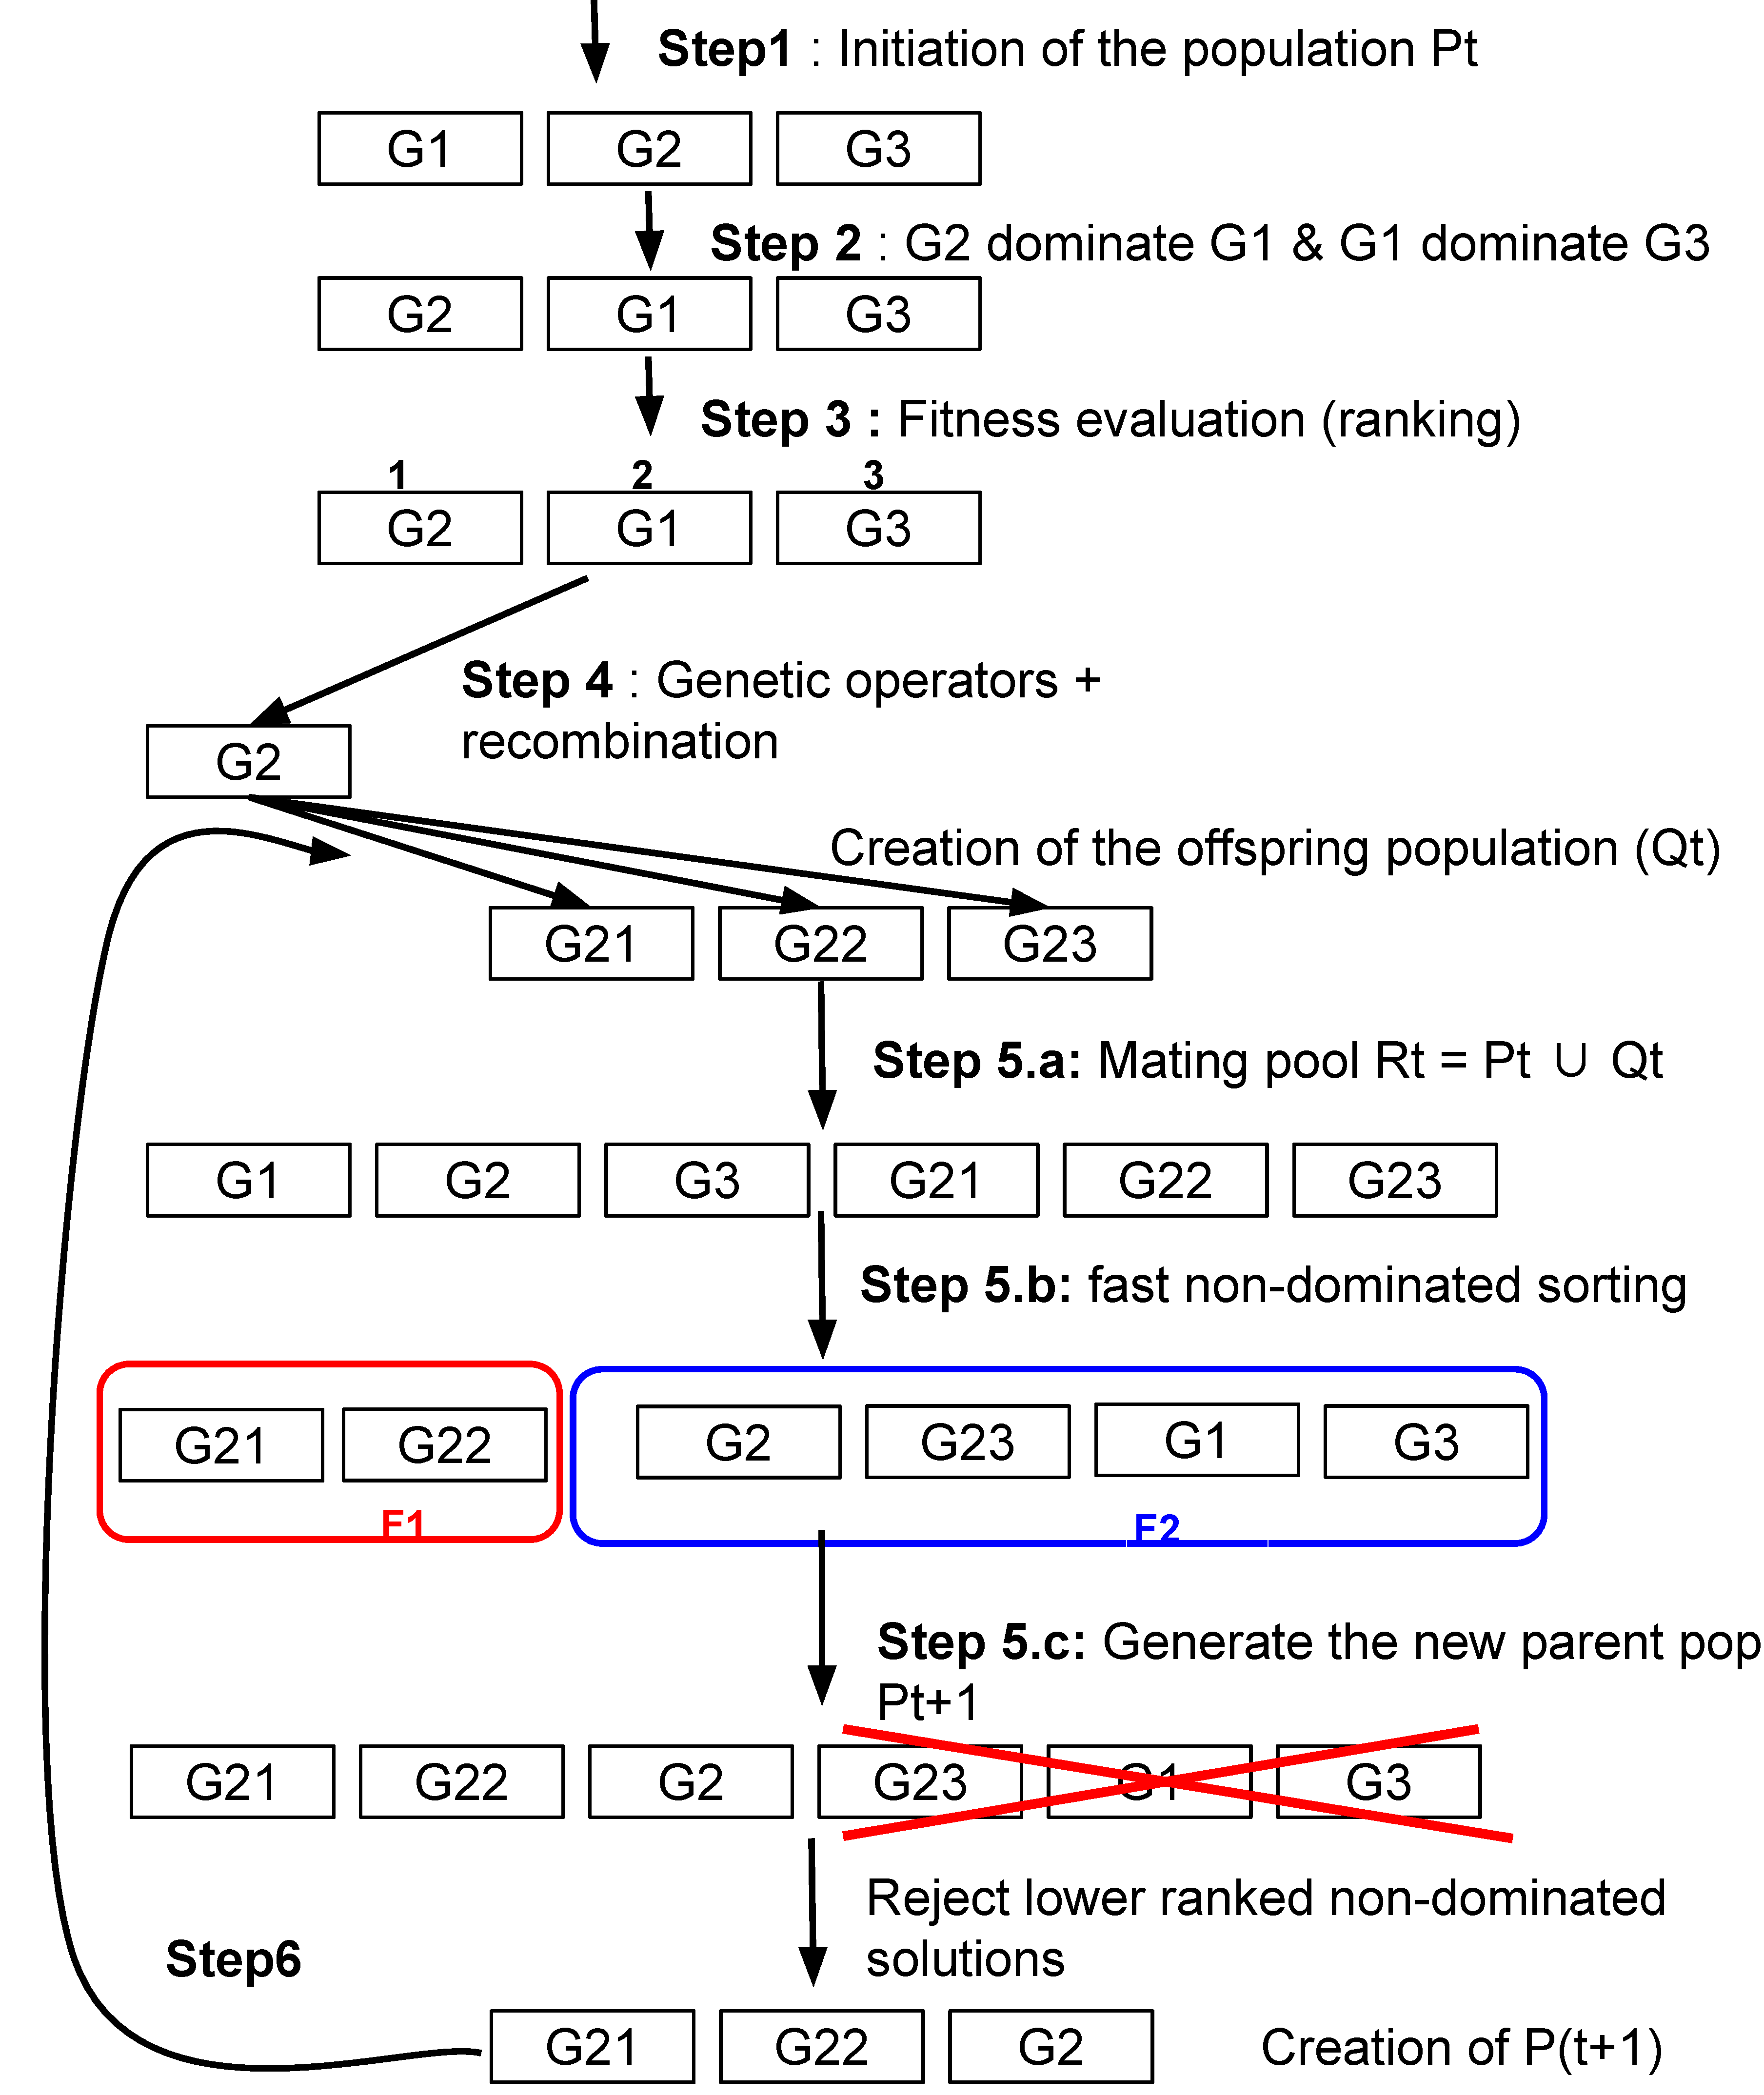
\includegraphics[width=3.49in]{NSGAII.pdf}
\caption{Schema of the NSGA-II algorithm}
\label{nsgaii}
\end{figure}

Figure~\ref{nsgaii} gives an overview of how to use NSGA-II to automate the exploration of complex systems design space. The steps of this algorithm are as follow :

\begin{enumerate}
\item Initially, Create a random parent population $P_{0}$ composed of N genomes (N = 3 in Figure~\ref{nsgaii}). N represent the size of the population.
\item Sort the current population based on a non domination criterion (e.g. reliability, availability and response time).
\item For each non-dominated solution, assign a fitness (rank) equal to its non-domination level (1 is the best level, 2 is the next best level, and so on).
\item Create a child population $Q_{0}$ of size N using binary tournament selection, recombination, and mutation operators.
\item From the first generation onwards, creation of each new generation constitutes the following steps :
\item[5.a)] Create the mating pool $R_{t}$ of size 2N by combining the parent population $P_{t}$ and the child population $Q_{t}$.
\item[5.b)] Sort the combined population $R_{t}$ according to the fast non-dominated sorting procedure to identify all non-dominated fronts $(F_{1} ,F_{2},...,F_{k})$.
\item[5.c)] Generate the new parent population $P_{t}+1$ of size N by adding non-dominated solutions starting from the first ranked non-dominated front $F1$ and proceeding with the subsequently ranked non-dominated fronts $F_{1} ,F_{2}, . . . ,F_{k}$, till the size exceeds N (Figure~\ref{nsgaii}). This means that the total count of the non-dominated solutions from the fronts $F_{1} ,F_{2}, . . . ,F_{k}$, exceeds the population size N. Now, in order to make the total count of the non-dominated solutions equal to N, it is required to \textbf{reject} some of the lower ranked non-dominated solutions from the last $Fkth$ front. This is achieved through a sorting process based on the crowding distance assigned to each solution contained in the $F_{k}th$ non-dominated front. Thus, the new parent population $P_{t}+1$ of size N is constructed.
\item Perform the selection, crossover and mutation operations on the newly generated parent population $(P_{t}+1)$ to create the new child population $(Q_{t}+1)$) of size N (Figure~\ref{nsgaii}).
\item Repeat Step 5 until a stopping criterion is met (e.g. maximum number of generations is reached).

\end{enumerate}


\section{Using evolutionary algorithms for identifying best design alternatives}
\label{Approach}
Figure~\ref{IS} graphically illustrates the approach proposed in this paper by showing the process underlying it. As can be seen in Figure~\ref{IS}, the process starts with an initial input software architecture which could be designed by software architects by using architecture design languages\cite{Medvidovic}. After that, the input model is transformed into a set of alternative architecture models (more detailed models) driven by a set of competing NFP. To solve the trade-off between NFP we expressed the architecture alternatives as design patterns implemented by means of model transformations and compositions techniques. The next step consists at finding the best model transformations alternatives. To do so we (i) map these model transformations alternatives as a multiple-objectives optimization problem and (ii) use NSGA-II to find the non-dominated solutions. 

%The final step in Figure~\ref{IS} consists in exploring the design space composed of all model transformation compositions and select which transformation fulfil at best the NFP of the system. This step is done by using an advanced evolutionary algorithm.

\begin{figure}[!ht]
\centering
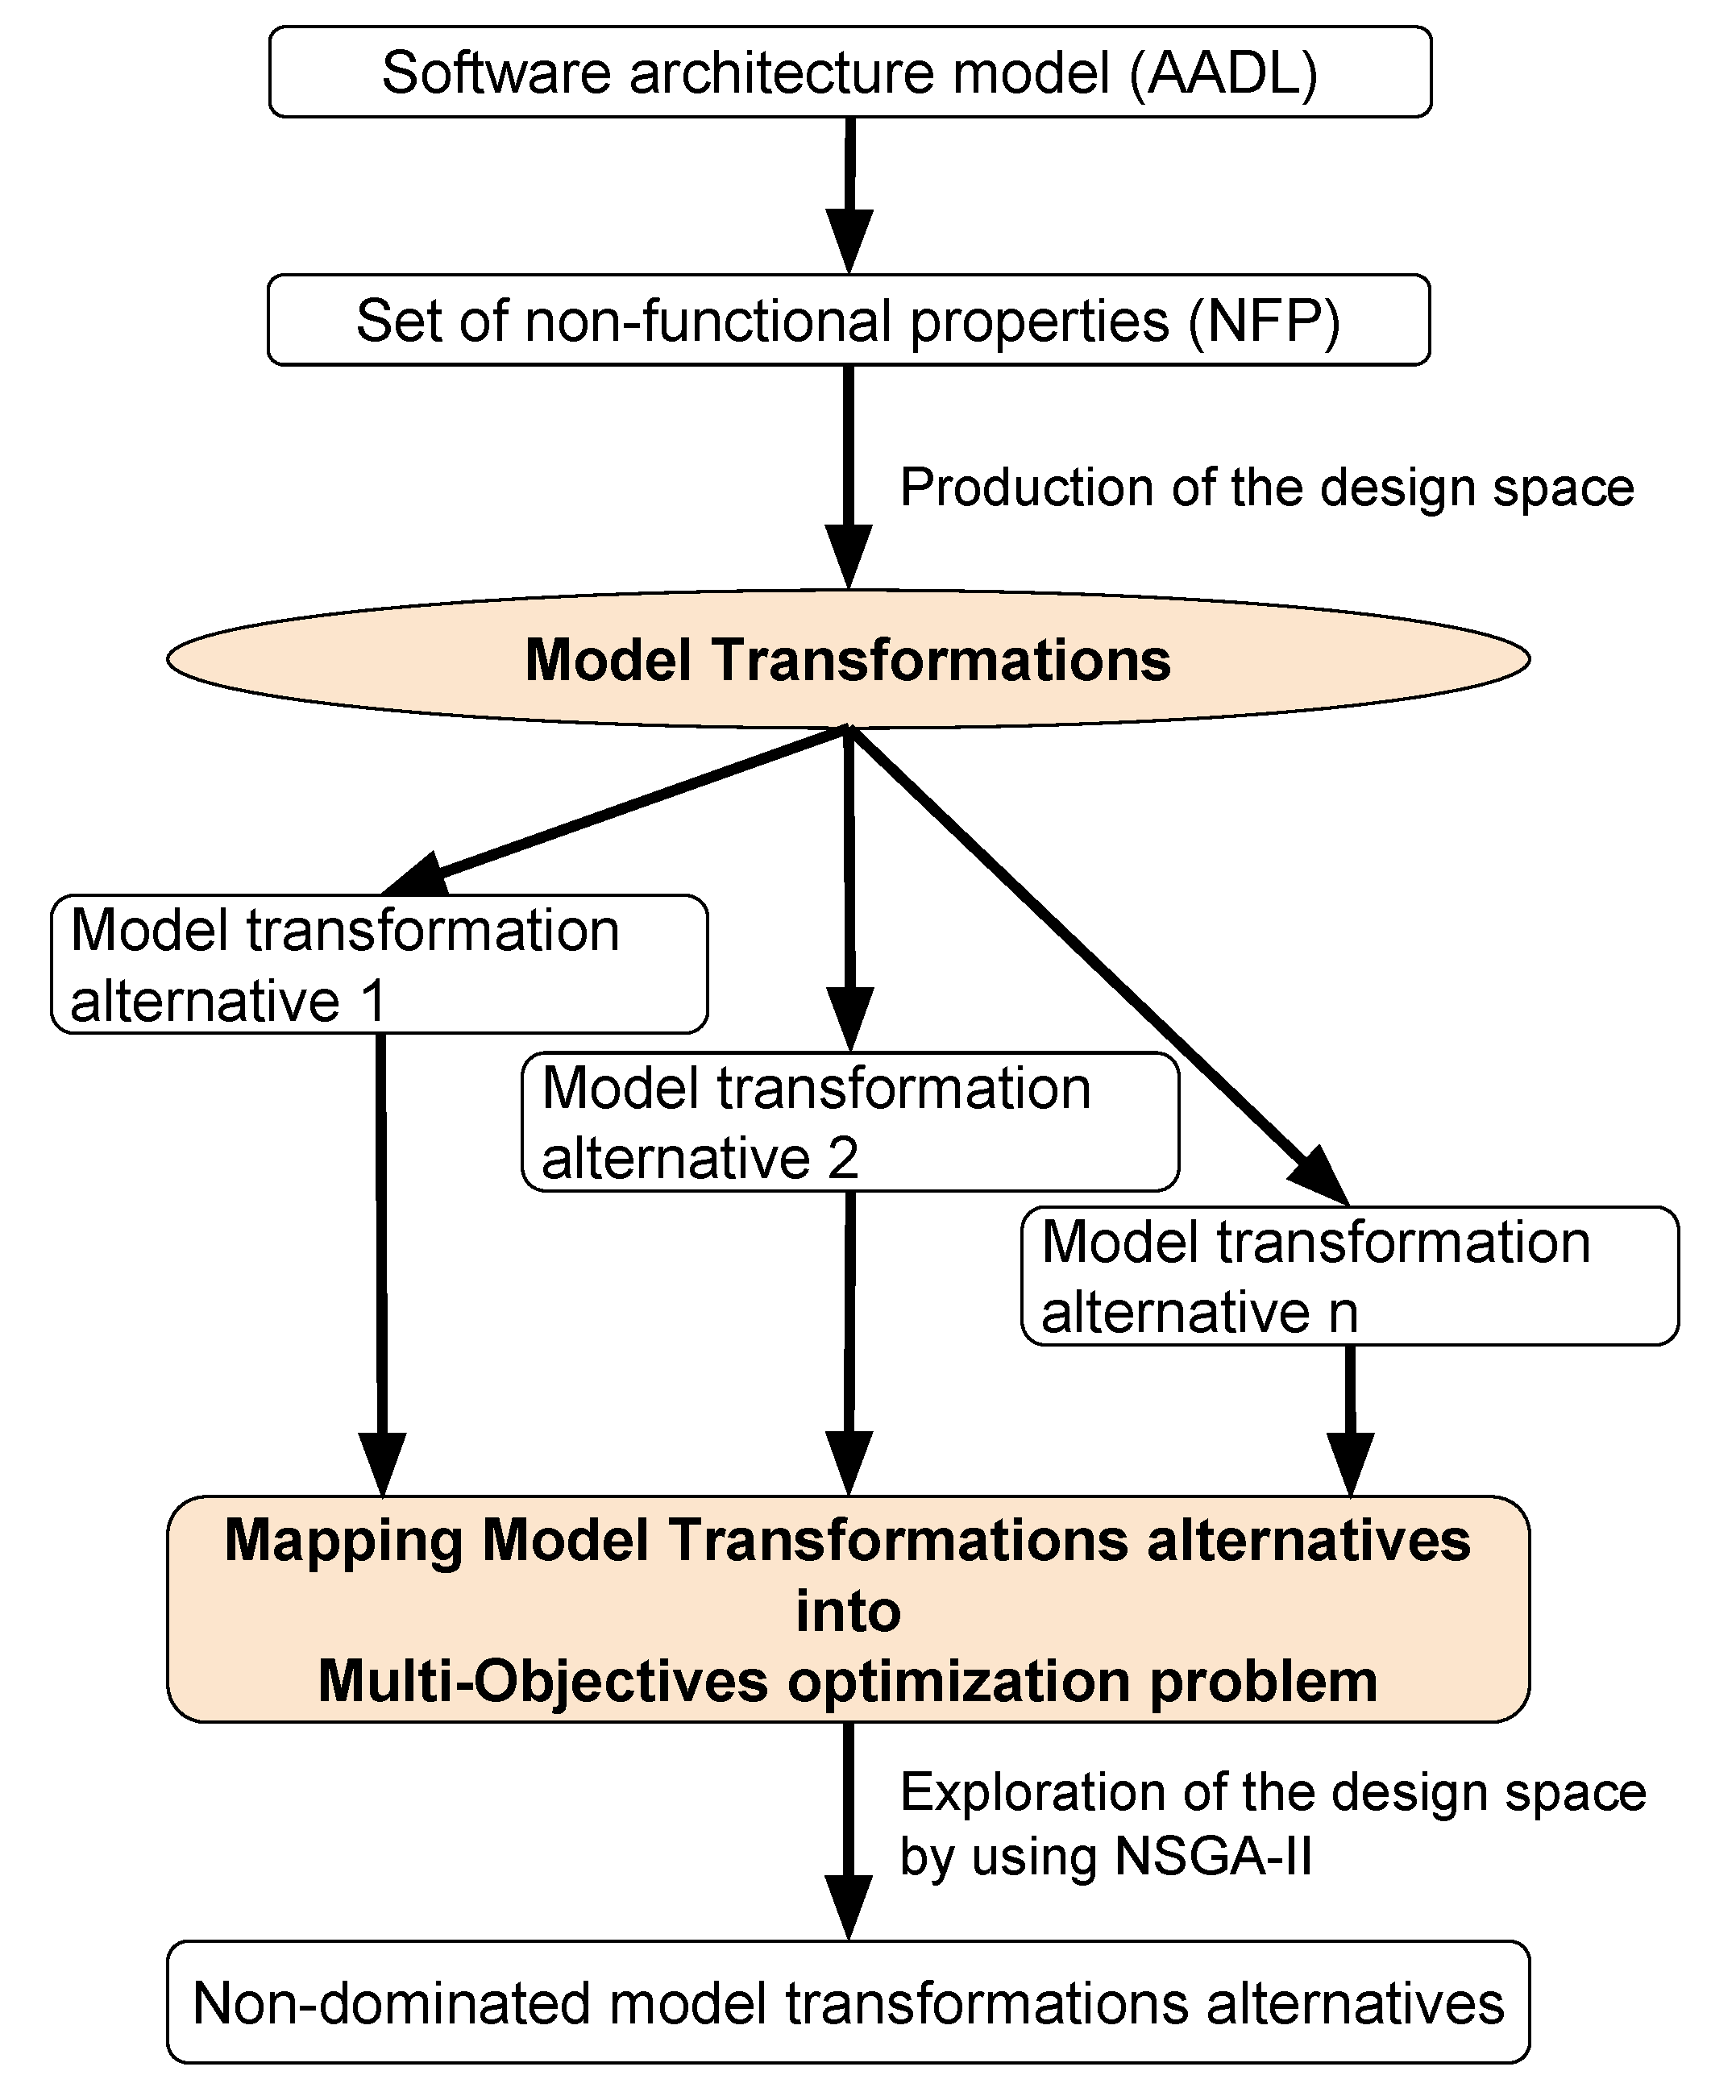
\includegraphics[width=3.49in]{IDMT.pdf}
\caption{Approach overview}
\label{IS}
\end{figure}

\subsection{System architecture modelisation}
Since our application domain is embedded systems, we have chosen AADL (Architecture Analysis \& Design Language) as the underlying architecture description language. AADL has been designed on the foundation of the architecture description language MetaH and its goals are (i) specification of quality analysis (e.g. safety); and (ii) design architectures for complex embedded systems. It offers a standardized semantics, mostly expressed using natural language and the components are composed hierarchically according to standardized composition rules. AADL also allows the designers to expand model by defining new property sets in their own specific way. The other reason of choosing AADL is to integrate our work in an existing framework RAMSES\footnote{Refinement of AADL Models for the Synthesis of Embdded Systems. \url{http://penelope.enst.fr/aadl/wiki/Projects}} which apply selection of design alternatives.

\subsection{Model transformations composition}
\label{transfos}
In major cases, model transformations are grouped into two main categories of model transformation languages : (i) rule-based transformation languages, or (ii) imperative transformation languages\cite{Gorp06integratinga}.

The first category express model transformation logics in a way that is easy to interpret and \textbf{adapt}. It permit to modify the pattern matching part of a transformation rule $TR$ which is sufficient to modify the set of elements this rule applies to. In contrary, the adaptation of imperative transformation languages are more difficult and requires a deep understanding of the control flow graph that leads to the execution of one or another transformation.

We used in our work the first category of languages since it more easy to adapt into other methods (in this paper MOEA). Where model transformations are endogenous : the source and target models are the same. In our work we use a AADL to AADL model transformations in order to improve (or refine) the architecture of an embedded system while representing the result of this refinement in an analysable model. More specific, we use the rule-based transformation language ATL (for Atlas Transformation Language).

A model transformation $MT$ is generally composed of a set of transformation rules $(TR_{i})$. Each transformation rule $TR_{i}$ is defined by a pair $<E_{j},R_{j}>$, where $E_{j}$ is the scope of the transformation rule $TR_{i}$ : the set of elements from the input model the transformation rule $TR_{i}$ can be applied to. And $R_{j}$ is the set of rules or actions which $TR_{i}$ executes when it is applied to an element of $E_{j}$ (i.e. creation of elements in the target model).

%In the second step of this approach, we use the rule-based transformation language ATL (for Atlas Transformation Language), where architecture alternatives are implemented as model transformations driven by NFPs. 

\subsection{Mapping model transformation alternatives into a multiple-objectives optimization problem}
\label{Adapting}
The next step of our approach consist in using model transformations definitions described in Section~\ref{transfos} and integrate them into a multiple-objectives optimization problem. Where the population to optimize or the design space represent a set of model transformations alternatives and the objectives to fulfils are NFP such as reliability, availability and response time. The integration process is described in the following sections.
\subsubsection{\textbf{Genome representation}}

\begin{figure}[!ht]
\centering
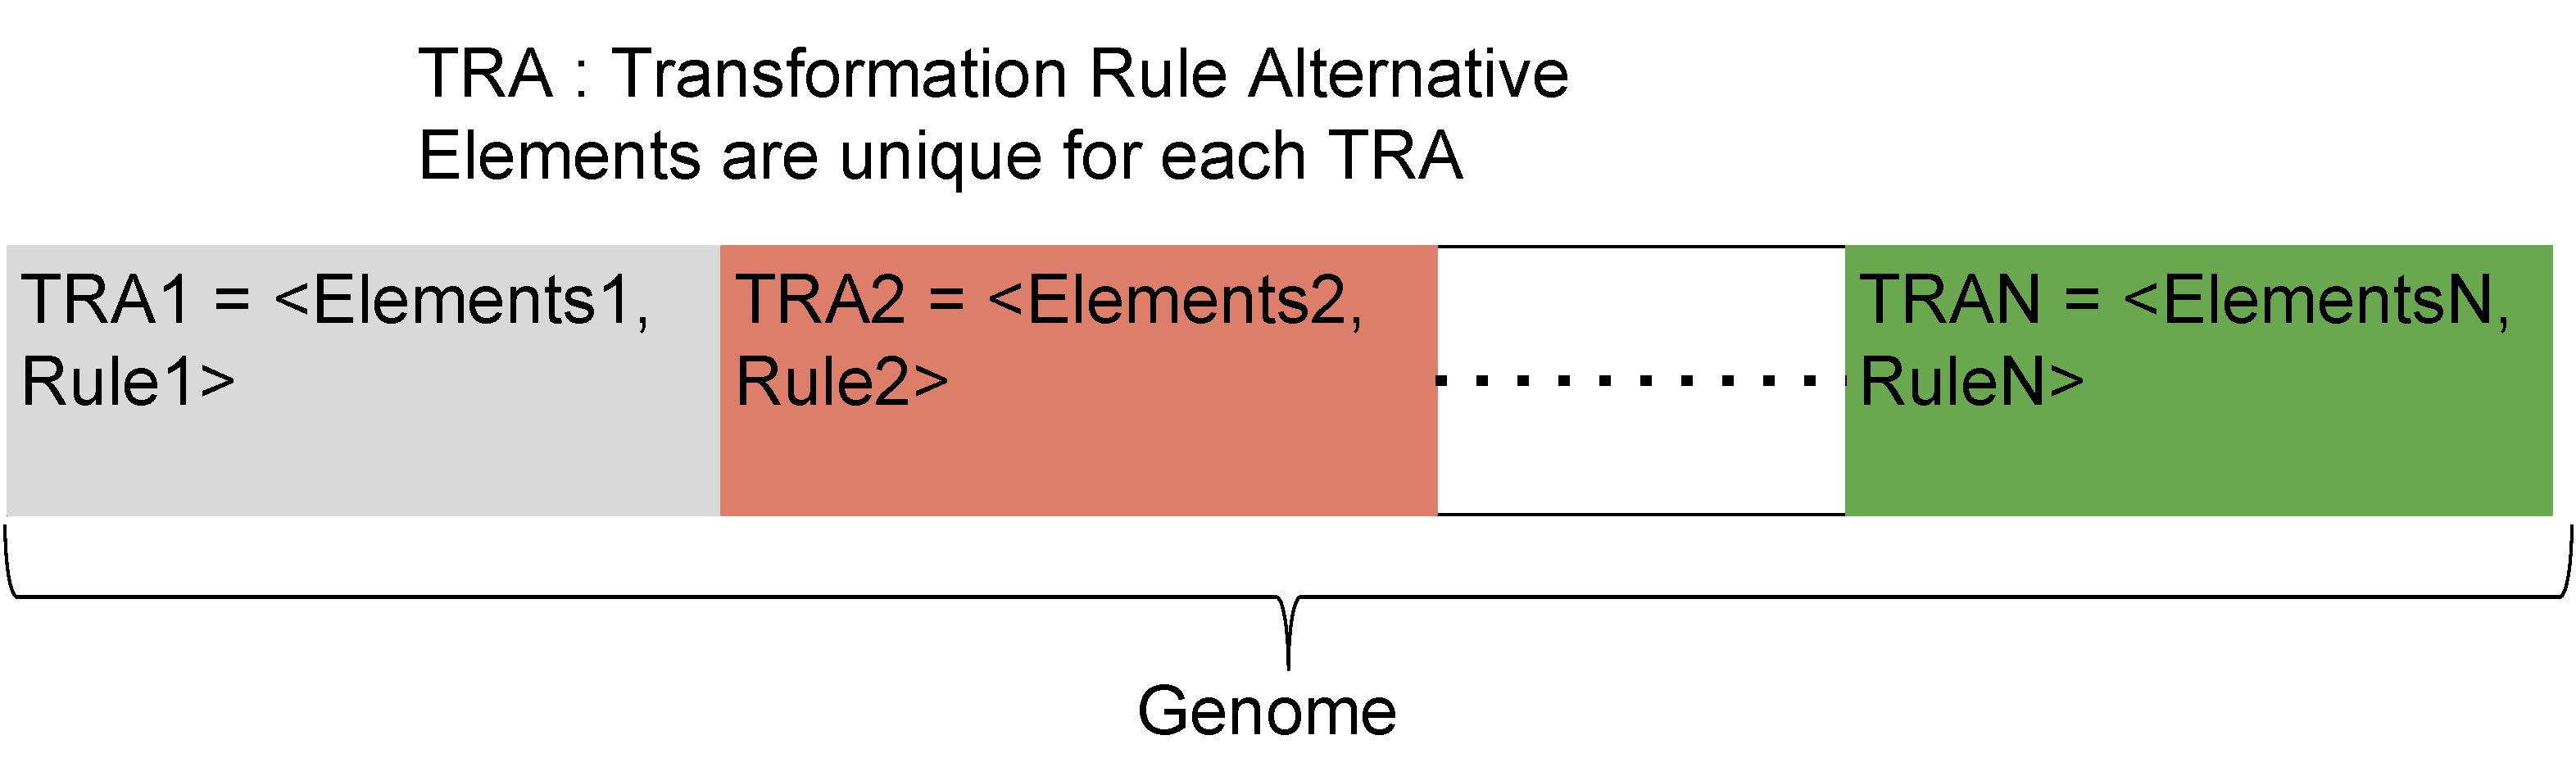
\includegraphics[width=3.49in]{genome.pdf}
\caption{Genome overview}
\label{genome}
\end{figure}

The major element to define in a multiple-objective optimization problem (MOOP) is the population to optimize. In our work, the population is a set of model transformations alternatives (MTA). Where each genome is a MTA and each gene represent the composition of this MTA.

Figure~\ref{genome} gives an overview of our mapping of a MOOP genome. A genome G represent a MTA and is composed of a sequences of genes. A gene is composed of a set of Transformation Rules Alternative (TRA). Each $TRA$ is, in turn, encoded as a pair $<Elements,Rule>$ where $Elements$ is a list of elements from the input model, and $Rule$ is a transformation rule which can be applied to $Elements$.

%Each genome $G_{i}, i \in {1,2,...,n}$ is composed of a set of TRA $(G = {TRA_{i}, i \in {1,2,...n}})$. Each $TRA_{i}$ is, in turn, encoded as a pair $TRA_{i} = <Elements_{i},Rule_{i}>$ where $Elements_{i} (i ={1,2,...,n})$ is a list of elements from the input model, and $Rule_{i} (i ={1,2,...,n})$ is a transformation rule which can be applied to $Elements_{i}$.

\subsubsection{\textbf{Fitness evaluation of each genome}}
In each generation, the fitness of every genome in the population is evaluated. The fitness is usually the value of the objective function in the optimization problem being solved. We defined in our work one fitness function corresponding to three objectives reliability, availability and response time.
The aim of our work is to maximize these three objectives. 

The more fit genomes are stochastically selected from the current population, and each genome is modified (recombined and possibly randomly mutated) to form a new generation.

\subsubsection{\textbf{Genetic operators}}
In NSGA-II, in each iteration, the N genomes selected from the previous generation are used to create new N genomes using genetic operators. This improves the existing solutions by mixing their genetic material (crossover) and/or by creating new material (mutation). Before applying the operators, the solutions are selected according to their fitness values, see Figure~\ref{nsgaii}. In our work, binary tournament selection, crossover and mutation operators are used.

\textbf{Binary tournament selection :} 
This operation consists of choosing some genomes at random in the population, and selecting the fittest two for reproduction. The selection criteria are the rank of the containing front and the crowding distance for solutions within the same front. Several tournaments are run to produce the needed genomes.

\begin{figure}[!ht]
\centering
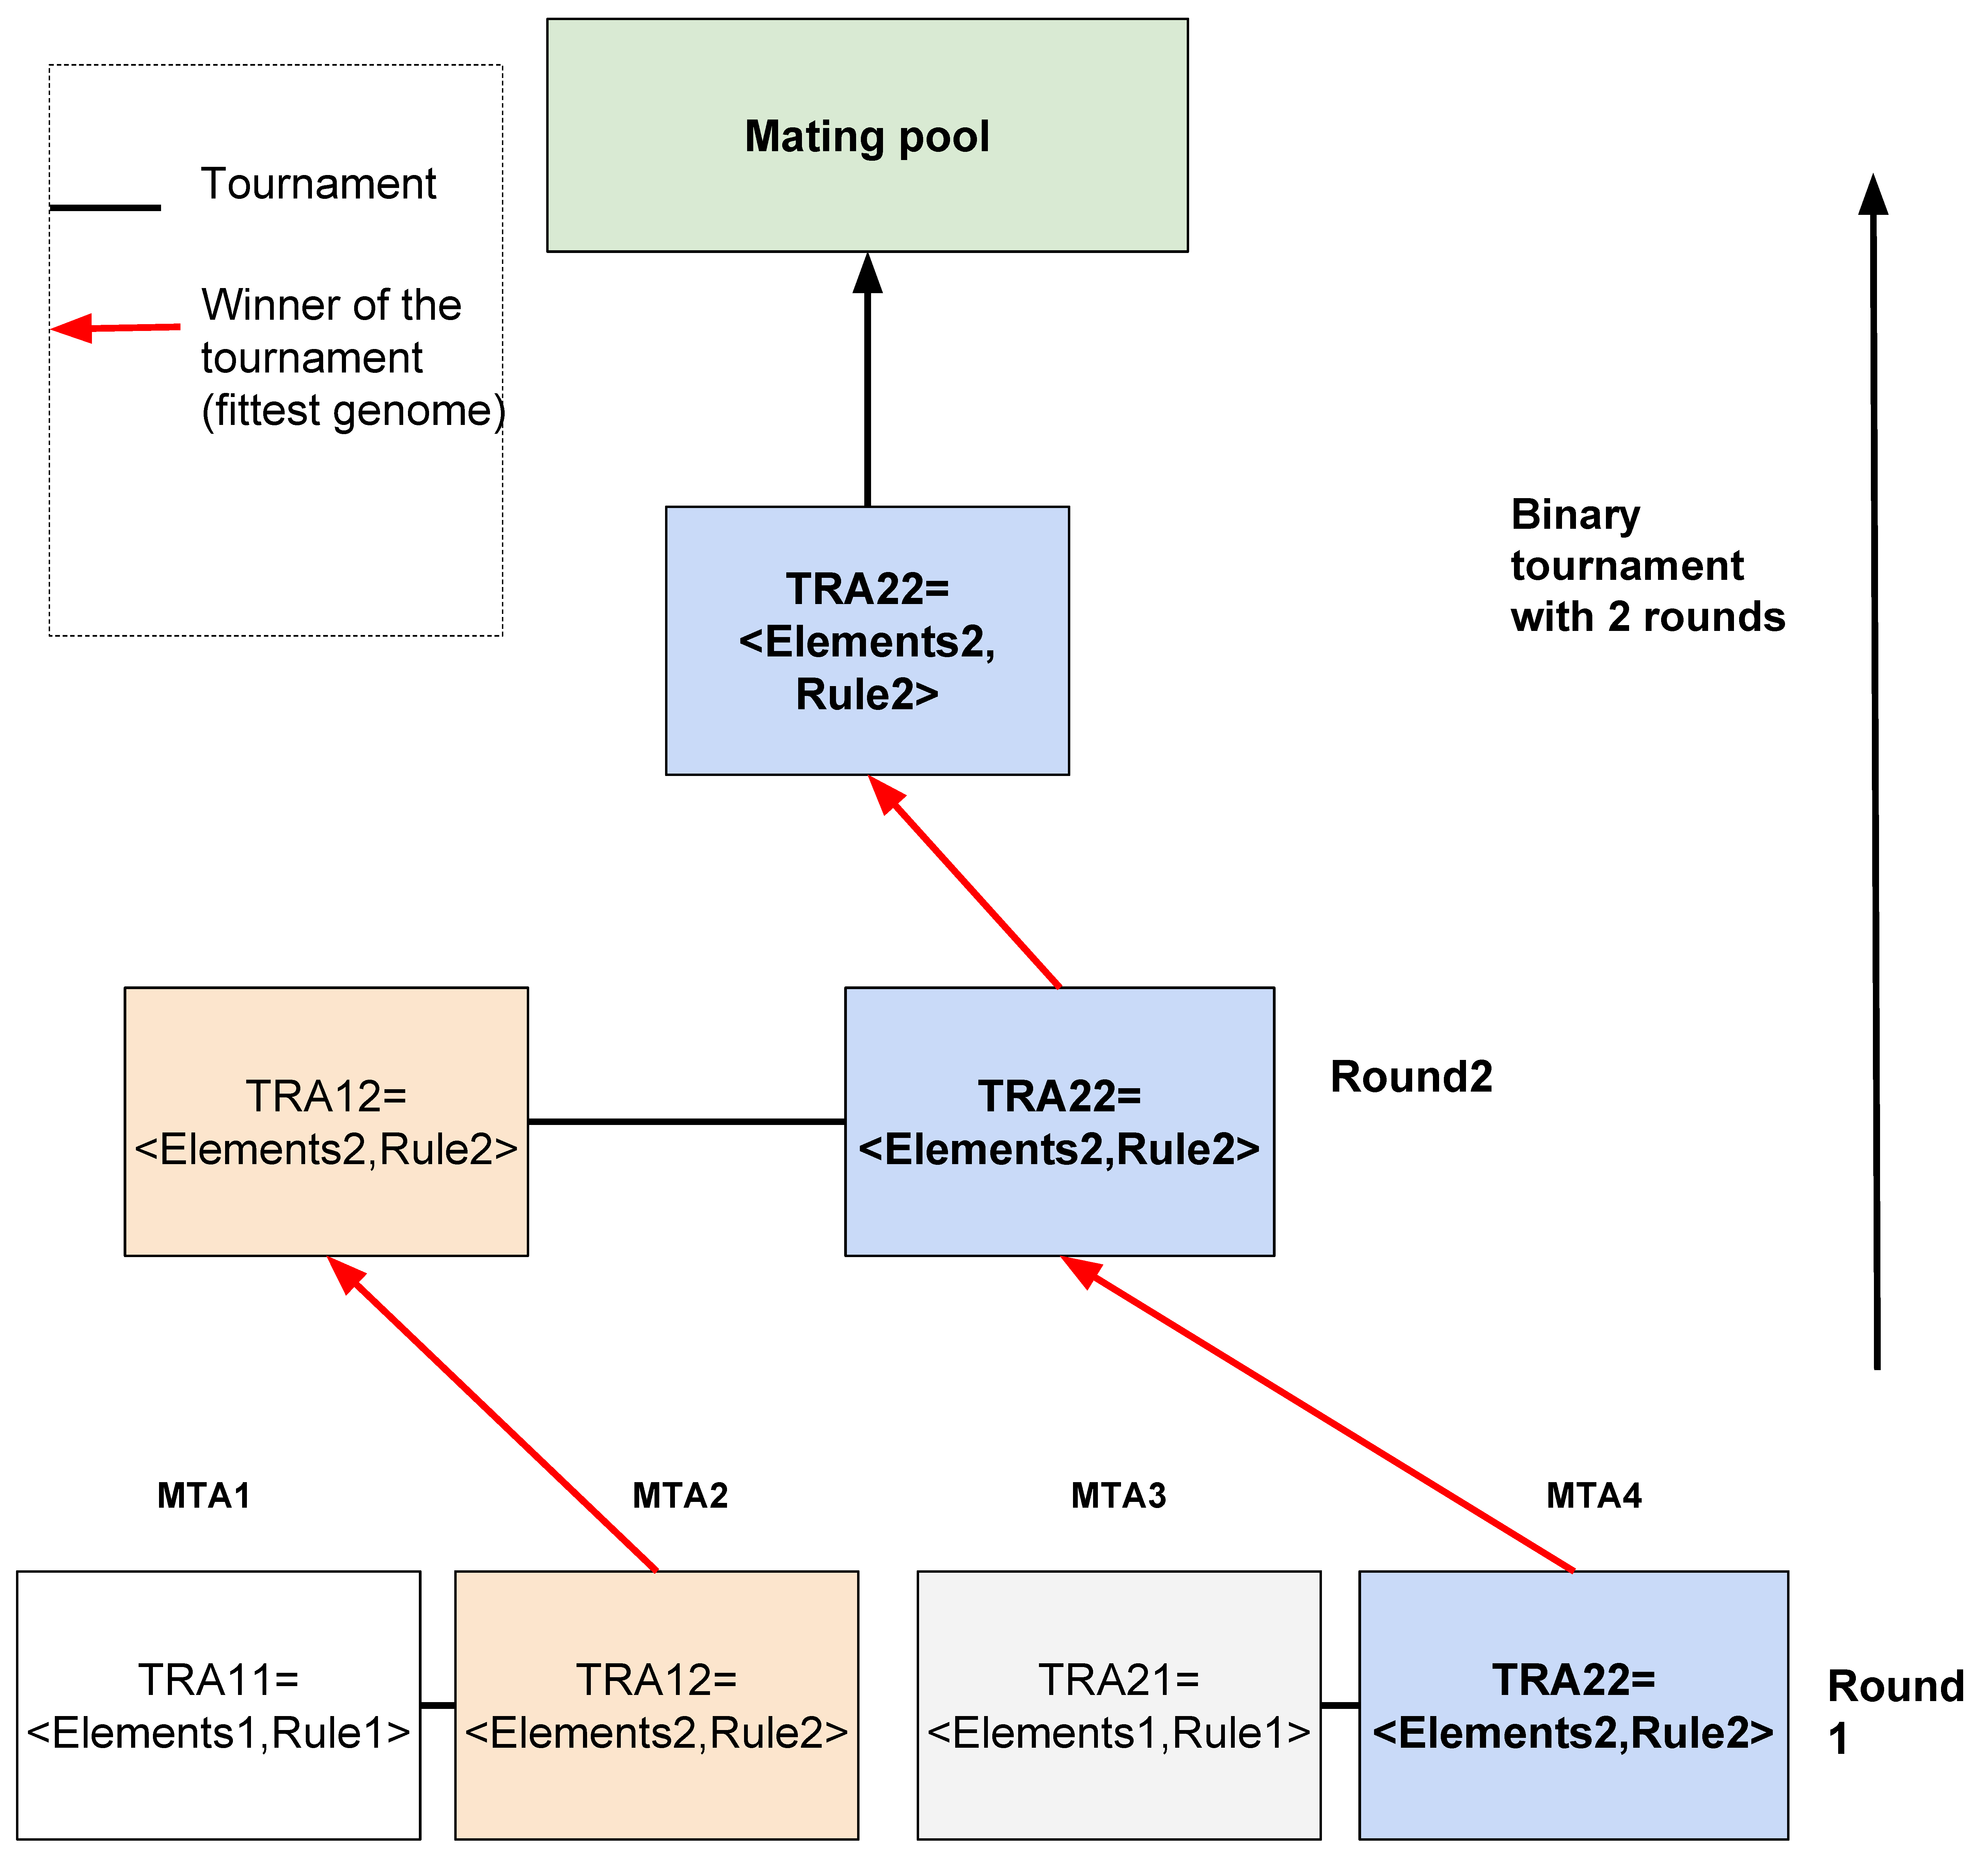
\includegraphics[width=3.49in]{bt.pdf}
\caption{Tournament Competition between Genomes}
\label{binary}
\end{figure}

Figure~\ref{binary} illustrates this operation. On this figure, we suppose we have four model transformations alternatives (genomes) MTA1, MTA2, MTA3 and MTA4 respectively composed of the following genes TRA11, TRA21, TRA31 and TRA41. We apply two tournaments between paired MTAs to produce the needed MTAs. In the first round we have two tournaments between two different pairs of MTAs (MTA1 with MTA2 and MTA3 with MTA4). In the second round we apply another tournament on the victorious MTAs in the previous round (MTA2 and MTA4) to get the fittest MTA which will be put in the mating pool for reproduction (generate new MTAs). In Figure~\ref{binary} the fittest MTA which is expected to appear in the mating pool is MTA4.

\textbf{Crossover :} 
The crossover consists of producing new genomes from the existing ones. When two genomes are selected using the binary tournament selection, two offspring solutions are created, with a given crossover probability, by exchanging parts of the parent genomes. This consists in randomly selecting a cut point in the genome, and all the genes beyond that point in either parent are swapped between the two parents.

\begin{figure}[!ht]
\centering
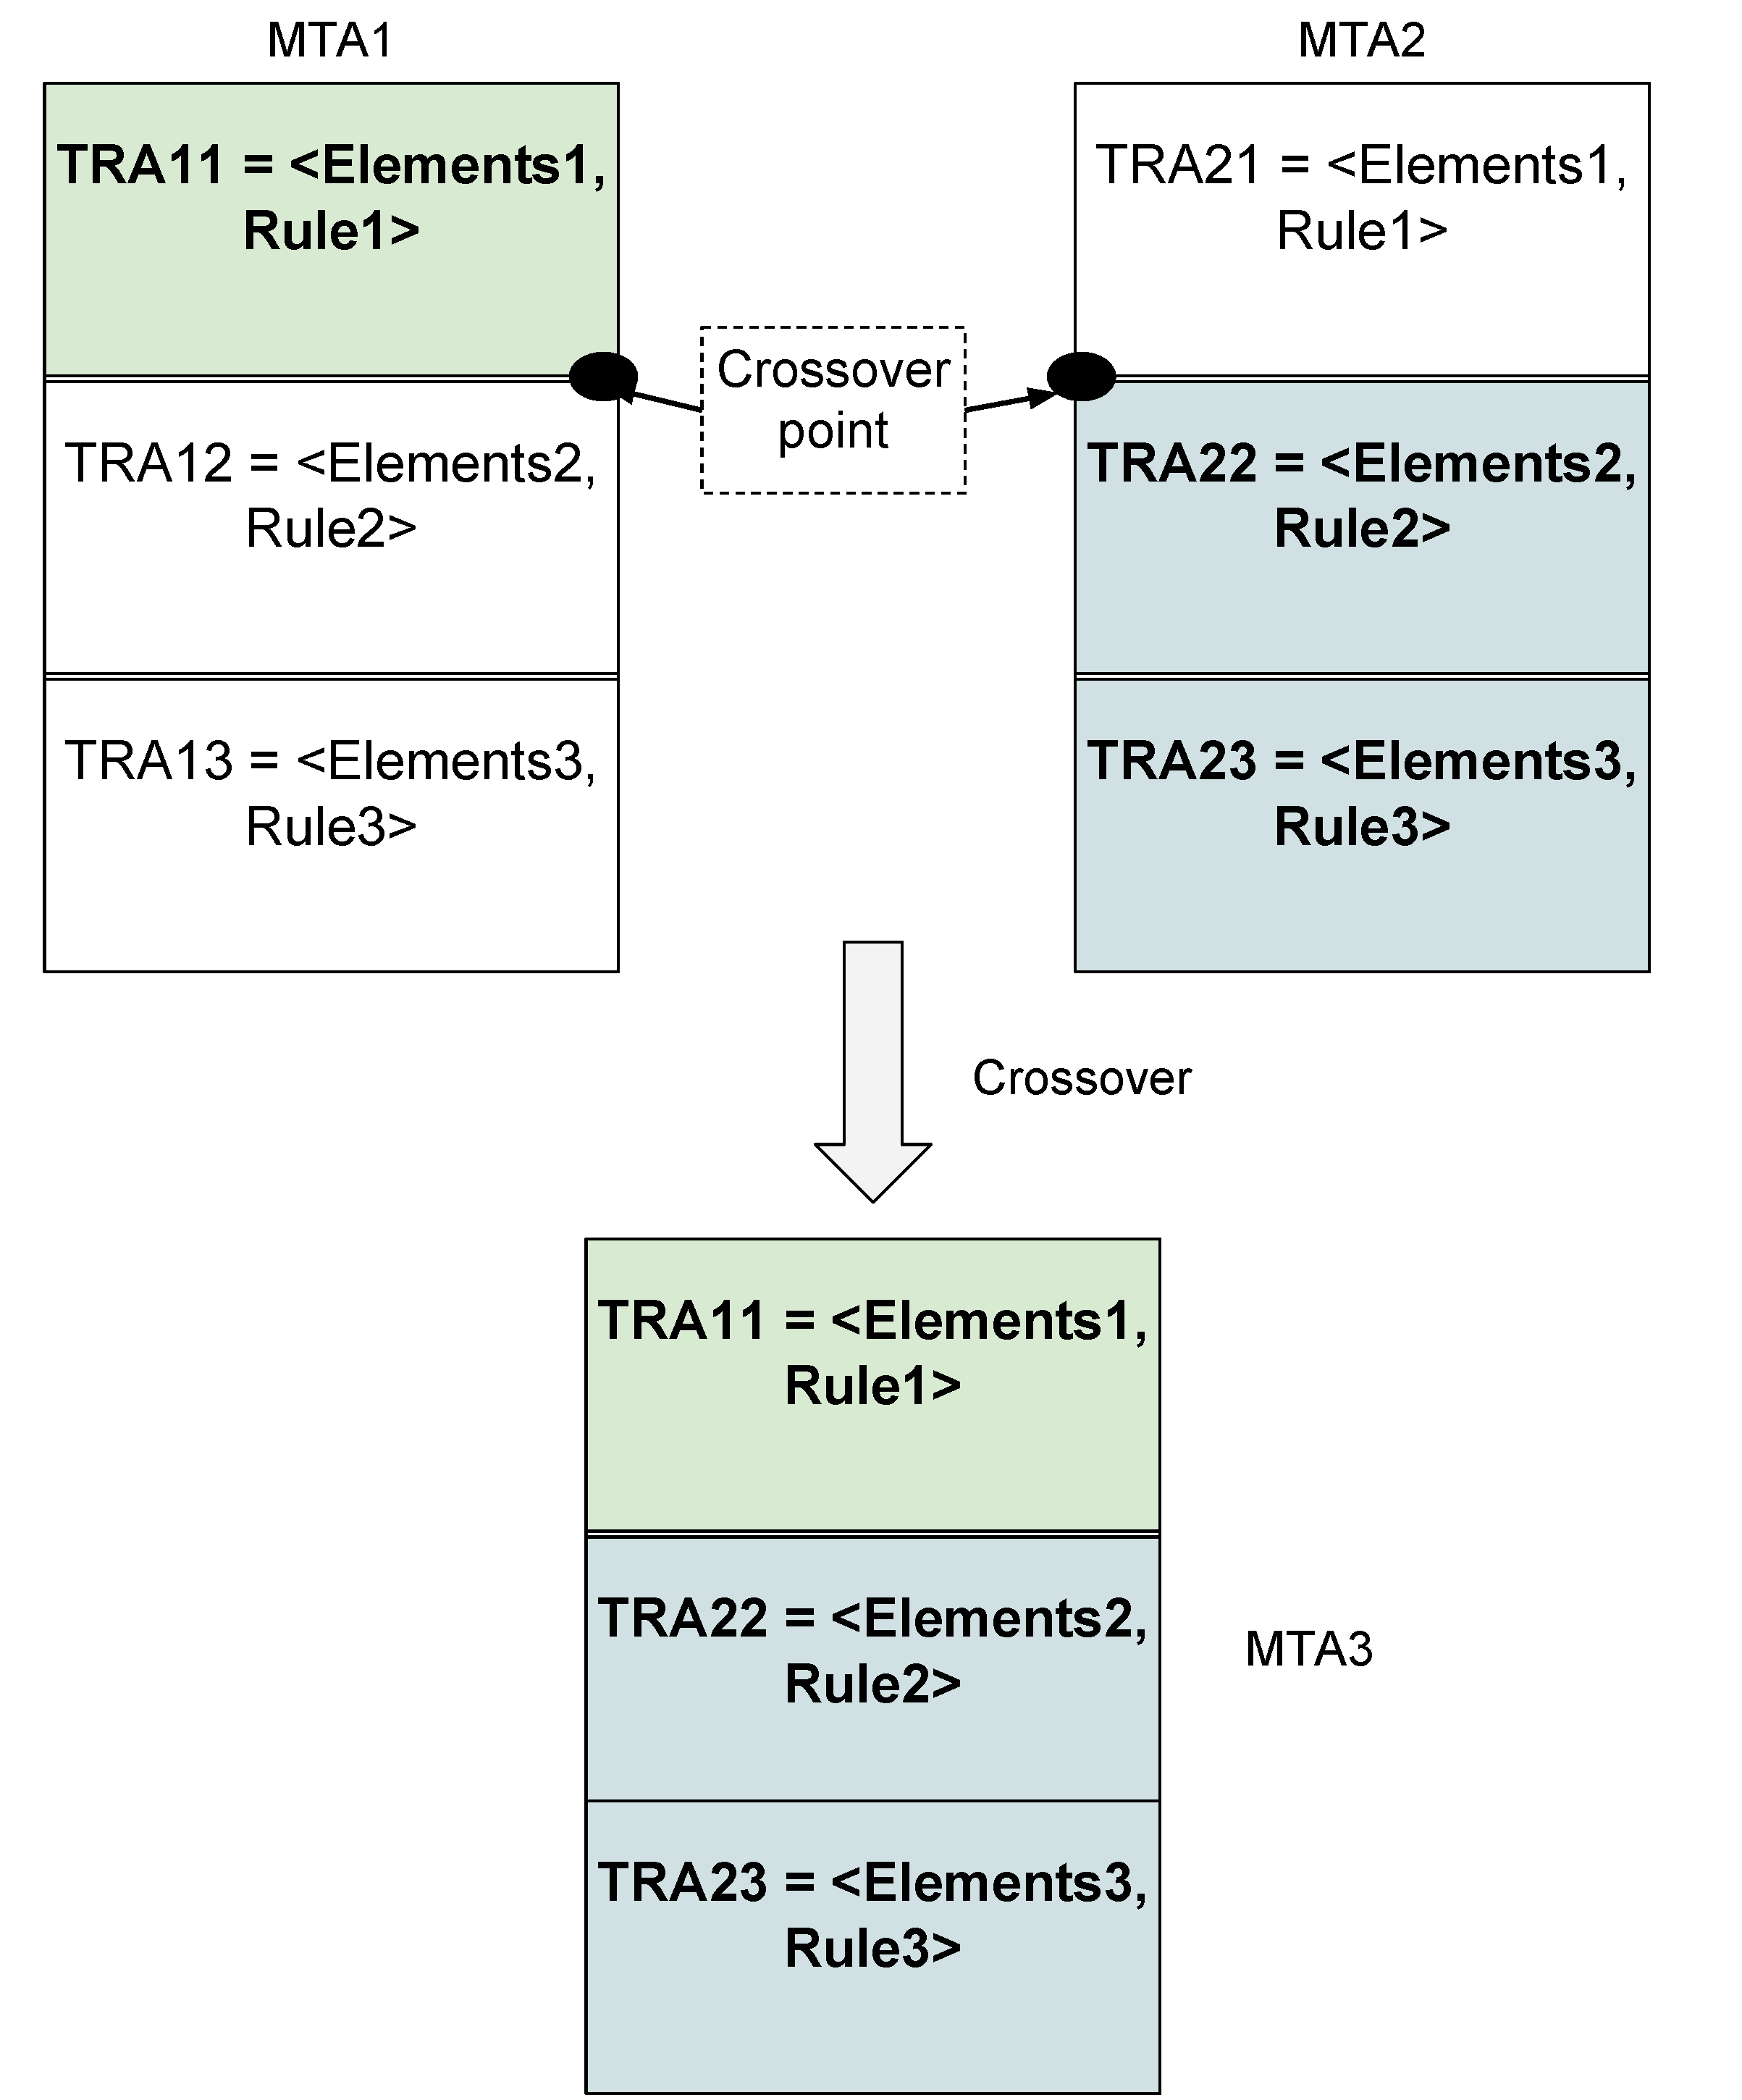
\includegraphics[width=3.49in]{crossover.pdf}
\caption{Crossover operator}
\label{crossover}
\end{figure}

Figure~\ref{crossover} illustrates the result of applying the crossover operator to two parent genomes MTA1 and MTA2 respectively composed of the following genes \{TRA11,TRA12,TRA13\} and \{TRA21,TRA22,TRA23\} to produce a new genome MTA3 composed of new sequence \{TRA11,TRA22,TRA23\}. As can be seen in Figure~\ref{crossover}, this operator combines TRA11 from MTA1 and {TRA22,TRA23} from MTA2 by selecting a single point on the genome and swapping the genes between the two genomes that lie beyond this point. 

\textbf{Mutation :}
After performing the crossover, the obtained solutions could be mutated with a given mutation probability.

\begin{figure}[!ht]
\centering
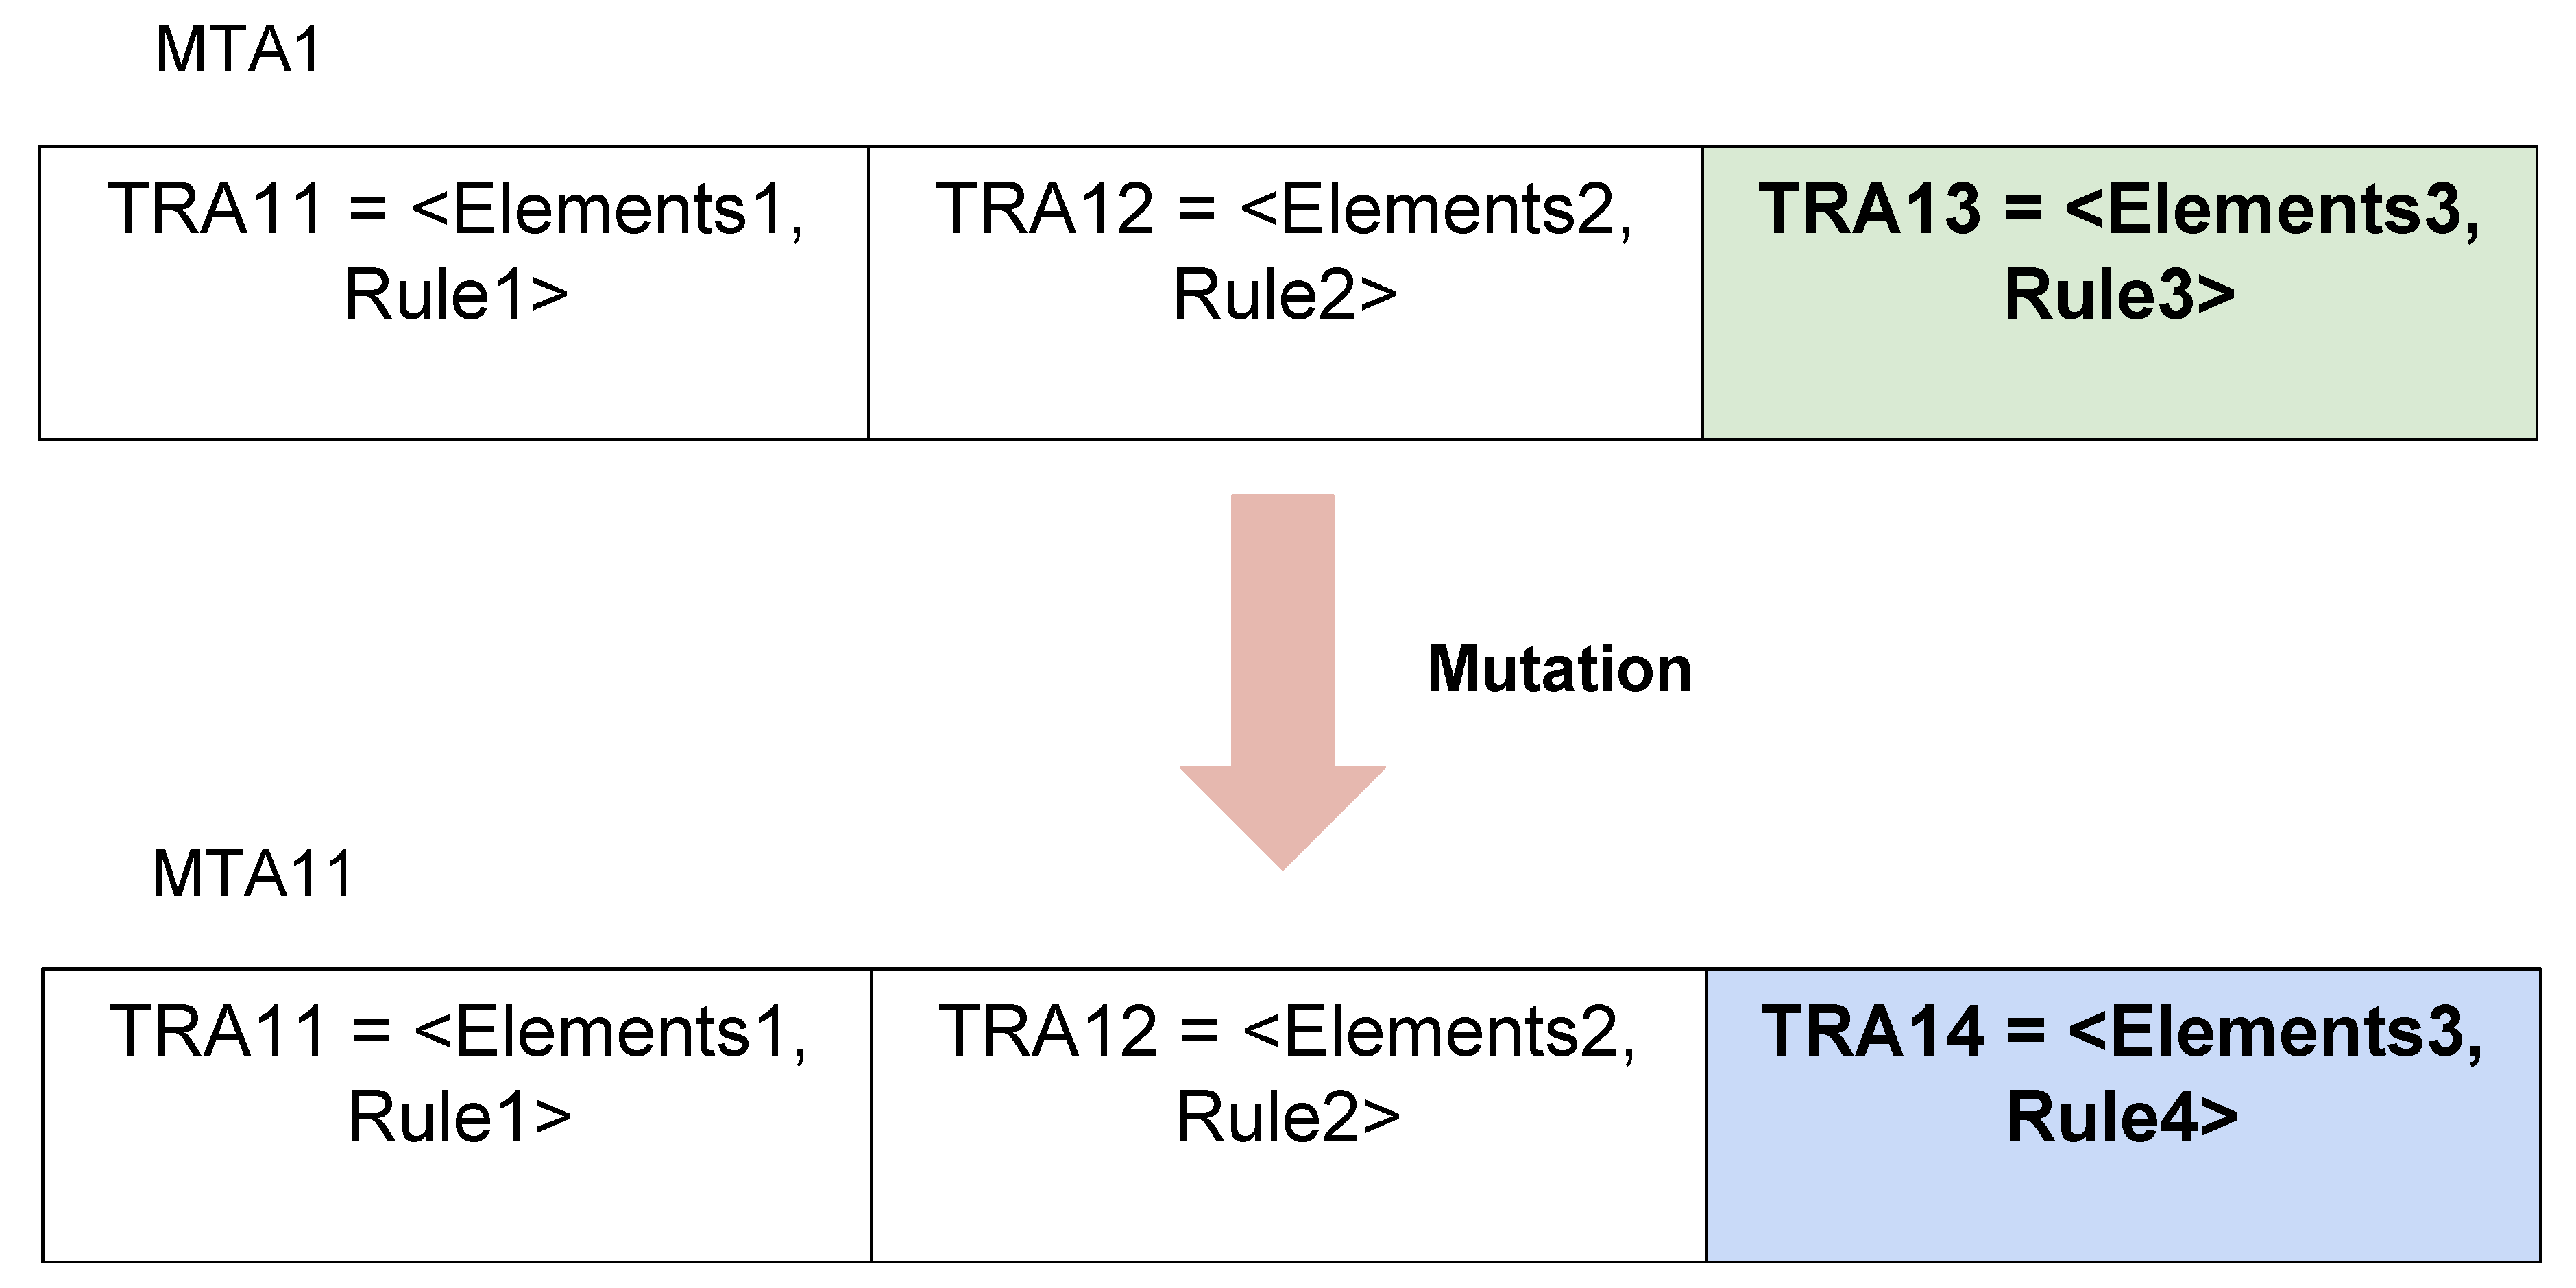
\includegraphics[width=3.49in]{mutation.pdf}
\caption{Mutation operator}
\label{mutation}
\end{figure}

The mutation operator act on a single genome MTA1 to obtained a muted genome MTA11 acts as follows. The mutation operator selects a gene at random in the genome and changes its value. In Figure~\ref{mutation}, the third gene TRA13 is selected to mutate into a new gene TRA14 : we apply a different rule (i.e. rule4) to the set of selected elements.

The final step of our approach consists in using the NSGA-II algorithm described in Section~\ref{nsgaii} to our optimization design problem defined above to find the set of non-dominated model transformations alternatives.

\section{Related Work}
\label{Related}
Our work is based on system performance prediction\cite{1291833} by using model transformations techniques and multi-objective metaheuristic optimization\cite{Coello98acomprehensive}.

\subsection{model transformations techniques}
Recently, some works have focused on the definition of model transformation alternatives. The first works introduced the superimposition mechanism\cite{Navarro:2011:UMT:2041790.2041840} to implement transformations alternatives. Another work\cite{Kavimandan:2011:MQS:2000259.2000264} proposed to implement transformations alternatives by using rule-based transformation languages. These works has been continued in\cite{Drago:2011} in order to deal with architecture quality problems. 

Our contribution is based on this work since it enable the factorization and composition of model transformations. However, this approach doesn't propose any algorithm to select the non-dominated (or pareto) model transformations alternatives which fulfil at best a set of competing non-functional properties.

\subsection{multi-objective metaheuristic optimization}
Aleti et al.\cite{Gr5069138} have developed the ArchOpteryx framework. ArchOpteryx assists the system architects during the design phase to create architectures that meet non-functional properties by using multi-objective optimization strategies. 

Koziolek et al.\cite{Koziolek:2011:PAA:2000259.2000267} also developed their own framework Peropteryx for improvement of system architecture models using a metaheuristic search guided by architectural tactics.

Unlike these two frameworks, in our approach design alternatives are implemented as model transformations driven by NFP. The use of model transformations help the design architects to (i) automating the system production; (ii) reusing architecture alternatives in other projects (or products) and (iii) solving the competition issue between NFP. 

Compared to DesignBots\cite{Diaz-Pace:2007:UPT:1784860.1784865}, in our method model transformations are not decomposed into subplans, each transformation is performed atomically.

For the optimization of NFP another work consists at using a cyclic process\cite{Bosch99softwarearchitecture}. The benefit of this process is its simplicity. The process can be tailored to different non-functional properties by using specific evaluation methods and architecture transformations. But this process focuses on only one non-functional property at a time unlike us who take into account several properties at a same time (e.g. reliability, availability and response time).

\section{Conclusion}
\label{Conclu}
An architecture design method has been presented that explicitly addresses the NFP put on the architecture. The proposed approach aims at improving system architecture models using two mechanisms. On the one hand, model transformations compositions to formalize model design alternatives. On the other hand, an elitist multiple-objective optimisation algorithm to explore this design space.

The main benefits of this approach is to handle a large search spaces of quality optimization problems and to automate the identification of good architecture design alternatives. This will reduce development costs and improve the quality of the final system. Additionally this approach enables the ranking of design alternatives with respect to conflicting NFP and the possibility to reuse these alternatives in other projects or products by reusing model transformations.

In the future, we plan to integrate our approach in the framework RAMSES and evaluating our approach in more details quantitatively (i.e. experimenting it on a an industrial case study)\cite{greg}.

\section{Acknowledgment}
This research work has been carried out under the leadership of the Technological Research Institute SystemX, and therefore granted with public funds within the scope of the French Program ``Investissements d'Avenir''.

\begin{thebibliography}{1}

\bibitem{Gr5069138}
A.~Aleti, S.~Bjornander, L.~Grunske, and I.~Meedeniya, ``Archeopterix: An
  extendable tool for architecture optimization of aadl models,'' in
  \emph{Model-Based Methodologies for Pervasive and Embedded Software, 2009.
  MOMPES '09. ICSE Workshop on}, May 2009, pp. 61--71.

\bibitem{1291833}
S.~Balsamo, A.~di~Marco, P.~Inverardi, and M.~Simeoni, ``Model-based
  performance prediction in software development: a survey,'' \emph{Software
  Engineering, IEEE Transactions on}, vol.~30, no.~5, pp. 295--310, May 2004.

\bibitem{Bosch99softwarearchitecture}
J.~Bosch, P.~Molin, J.~Bosch, and P.~Molin, ``Software architecture design:
  Evaluation and transformation,'' in \emph{In 1999 IEEE Engineering of
  Computer Based Systems Symposium. IEEE Computer Based Systems}, 1999, 
  pp. 4--10.

\bibitem{Coello98acomprehensive}
C.~A.~C. Coello, ``A comprehensive survey of evolutionary-based multiobjective
  optimization techniques,'' \emph{Knowledge and Information Systems}, vol.~1,
  pp. 269--308, 1998.

\bibitem{Deb:2002:FEM:2221359.2221582}
K.~Deb, A.~Pratap, S.~Agarwal, and T.~Meyarivan, ``A fast and elitist
  multiobjective genetic algorithm: Nsga-ii,'' \emph{Trans. Evol. Comp},
  vol.~6, no.~2, pp. 182--197, Apr. 2002. [Online]. Available:
  \url{http://dx.doi.org/10.1109/4235.996017}

\bibitem{Deb:2001:MOU:559152}
K.~Deb and D.~Kalyanmoy, \emph{Multi-Objective Optimization Using Evolutionary
  Algorithms}.\hskip 1em plus 0.5em minus 0.4em\relax New York, NY, USA: John
  Wiley \&amp; Sons, Inc., 2001.
 
\bibitem{Diaz-Pace:2007:UPT:1784860.1784865}
J.~A. D\'{\i}az-Pace and M.~R. Campo, ``Using planning techniques to assist
  quality-driven architectural design exploration,'' in \emph{Proceedings of
  the Quality of Software Architectures 3rd International Conference on
  Software Architectures, Components, and Applications}, ser. QoSA'07.\hskip
  1em plus 0.5em minus 0.4em\relax Berlin, Heidelberg: Springer-Verlag, 2007,
  pp. 33--52. [Online]. Available:
  \url{http://dl.acm.org/citation.cfm?id=1784860.1784865}

\bibitem{Drago:2011}
M.~Drago, C.~Ghezzi, and R.~Mirandola, ``Towards quality driven exploration of
  model transformation spaces,'' in \emph{Model Driven Engineering Languages
  and Systems}, ser. Lecture Notes in Computer Science, J.~Whittle, T.~Clark,
  and T.~Kühne, Eds., vol. 6981.\hskip 1em plus 0.5em minus 0.4em\relax
  Springer Berlin Heidelberg, 2011, pp. 2--16. [Online]. Available:
  \url{http://dx.doi.org/10.1007/978-3-642-24485-8_2}

\bibitem{Gorp06integratinga}
P.~V. Gorp, O.~Muliawan, D.~Janssens, P.~V. Gorp, O.~Muliawan, and D.~Janssens,
  ``Integrating a declarative with an imperative model transformation
  language,'' 2006.

\bibitem{greg}
G.~Loniewski, E.~Borde, D.~Blouin and E.Insfran {\'{}}, ``An Automated Approach for Architectural Model
  Transformations,'' in \emph{Information Systems
  Development, 22nd International Conference, {ISD} 2013,
  Sevilla, Spain, September 2013. Proceedings}, 2013, pp. 295-306.
  [Online]. Available: \url{http://infres.enst.fr/~borde/isd2013loniewski.pdf}

\bibitem{Johnsen1753}
A.~Johnsen and K.~Lundqvist, ``Developing dependable software-intensive
  systems: Aadl vs. east-adl,'' in \emph{Ada-Europe 2011}, A.~Romanovsky and
  T.~Vardanega, Eds.\hskip 1em plus 0.5em minus 0.4em\relax Springer-Verlag,
  June 2011, pp. 103--117. [Online]. Available:
  \url{http://www.es.mdh.se/publications/1753-}

\bibitem{Jouault:2005:TMA:2153686.2153705}
F.~Jouault and I.~Kurtev, ``Transforming models with atl,'' in
  \emph{Proceedings of the 2005 International Conference on Satellite Events at
  the MoDELS}, ser. MoDELS'05.\hskip 1em plus 0.5em minus 0.4em\relax Berlin,
  Heidelberg: Springer-Verlag, 2006, pp. 128--138. 
  [Online]. Available:  \url{http://dx.doi.org/10.1007/11663430_14}  

\bibitem{Kavimandan:2011:MQS:2000259.2000264}
A.~Kavimandan, A.~Gokhale, G.~Karsai, and J.~Gray, ``Managing the quality of
  software product line architectures through reusable model transformations,''
  in \emph{Proceedings of the Joint ACM SIGSOFT Conference -- QoSA and ACM
  SIGSOFT Symposium -- ISARCS on Quality of Software Architectures -- QoSA and
  Architecting Critical Systems -- ISARCS}, ser. QoSA-ISARCS '11.\hskip 1em
  plus 0.5em minus 0.4em\relax New York, NY, USA: ACM, 2011, pp. 13--22.
  [Online]. Available: \url{http://doi.acm.org/10.1145/2000259.2000264}
  
\bibitem{Kleppe2003}
A.~G. Kleppe, J.~Warmer, and W.~Bast, \emph{MDA Explained: The Model Driven
  Architecture: Practice and Promise}.\hskip 1em plus 0.5em minus 0.4em\relax
  Boston, MA, USA: Addison-Wesley Longman Publishing Co., Inc., 2003.

\bibitem{Koziolek:2011:PAA:2000259.2000267}
A.~Koziolek, H.~Koziolek, and R.~Reussner, ``Peropteryx: Automated application
  of tactics in multi-objective software architecture optimization,'' in
  \emph{Proceedings of the Joint ACM SIGSOFT Conference -- QoSA and ACM SIGSOFT
  Symposium -- ISARCS on Quality of Software Architectures -- QoSA and
  Architecting Critical Systems -- ISARCS}, ser. QoSA-ISARCS '11.\hskip 1em
  plus 0.5em minus 0.4em\relax New York, NY, USA: ACM, 2011, pp. 33--42.
  [Online]. Available: \url{http://doi.acm.org/10.1145/2000259.2000267}

\bibitem{Medvidovic}
N.~Medvidovic and R.~N. Taylor, ``A classification and comparison framework for
  software architecture description languages,'' \emph{IEEE Trans. Softw.
  Eng.}, vol.~26, no.~1, pp. 70--93, Jan. 2000. [Online]. Available:
  \url{http://dx.doi.org/10.1109/32.825767}

\bibitem{Navarro:2011:UMT:2041790.2041840}
E.~Navarro, C.~E. Cuesta, D.~E. Perry, and C.~Roda, ``Using model
  transformation techniques for the superimposition of architectural styles,''
  in \emph{Proceedings of the 5th European Conference on Software
  Architecture}, ser. ECSA'11.\hskip 1em plus 0.5em minus 0.4em\relax Berlin,
  Heidelberg: Springer-Verlag, 2011, pp. 379--387. [Online]. Available:
  \url{http://dl.acm.org/citation.cfm?id=2041790.2041840}

\bibitem{Srinivas94multiobjectiveoptimization}
N.~Srinivas and K.~Deb, ``Multiobjective optimization using nondominated
  sorting in genetic algorithms,'' \emph{Evolutionary Computation}, vol.~2, 
  pp. 221--248, 1994.

\bibitem{Tisi:conf/ecmdafa/TisiJFCB09}
M.~Tisi, F.~Jouault, P.~Fraternali, S.~Ceri, and J.~B{\'{e}}zivin, ``On the use
  of higher-order model transformations,'' in \emph{Model Driven Architecture -
  Foundations and Applications, 5th European Conference, {ECMDA-FA} 2009,
  Enschede, The Netherlands, June 23-26, 2009. Proceedings}, 2009, pp. 18--33.
  [Online]. Available: \url{http://dx.doi.org/10.1007/978-3-642-02674-4_3}

\bibitem{Yu:2001:CLA:502059.502038}
H.~Yu and A.~Vahdat, ``The costs and limits of availability for replicated
  services,'' \emph{SIGOPS Oper. Syst. Rev.}, vol.~35, no.~5, pp. 29--42, Oct.
  2001. [Online]. Available: 
  \url{http://doi.acm.org/10.1145/502059.502038}

\bibitem{Zitzler01spea2:improving}
E.~Zitzler, M.~Laumanns, and L.~Thiele, ``Spea2: Improving the strength pareto
  evolutionary algorithm,'' Tech. Rep., 2001.

\bibitem{Zitzler04indicatorbasedselection}
E.~Zitzler and S.~Künzli, ``Indicator-based selection in multiobjective
  search,'' in \emph{in Proc. 22nd International Conference on Information Systems
  Development (ISD 2013}.\hskip 1em plus 0.5em minus 0.4em\relax
  Springer, 2004, pp. 832--842.

\end{thebibliography}

\end{document}